% Template LaTeX document for CSSR4Africa Deliverables
% Adapted from documents prepared by EPFL for the RobotCub project
% and subsequently by the University of Skövde for the DREAM project
%
% DV 28/06/2023

\documentclass{CSSRforAfrica}

\usepackage[hidelinks,colorlinks=false]{hyperref}
\usepackage[titletoc,title]{appendix}
\usepackage{latexsym}

\usepackage{ragged2e}
\usepackage{dirtree}
\usepackage{listings}
\usepackage{textcomp}
\usepackage{multicol}
\usepackage{cprotect}
\usepackage{verbatim} % for comments
%\usepackage{xcolor}
\usepackage[dvipsnames]{xcolor}

\newcommand{\blank}{~\\}
\newcommand{\checkbox}{{~~~~~~~\leavevmode \put(-7,-1.5){  \huge $\Box$  }}}

\begin{document}
\input{epsf}

%%
%% SHOULD NOT NEED TO BE CHANGED BEFORE THIS POINT
%% ------------------------------------------------
%%

\deliverable{D3.2}                    
\title{D3.2 Software Engineering Standards Manual}

\leadpartner{Carnegie Mellon University Africa}                         
\partner{}                          

\revision{1.10}                  
\deliverabledate{30/09/2023}    
\submissiondate{26/10/2023}   
\revisiondate{13/09/2024}   
\disseminationlevel{PU}
\responsible{D. Vernon }            


%%
%% Create the titlepage
%%

\maketitle
 

\section*{Executive Summary}
%===============================================================
\label{executive_summary}
%%\addcontentsline{toc}{section}{Executive Summary}
 
Deliverable D3.2 is a reference manual of software engineering standards. 
It is based on the software engineering standards manual that was written for the EU-funded DREAM project \cite{DREAM}, Deliverable D3.2 \cite{DREAM3.2}, which was in turn based on the software engineering standards manual that was written for the EU-funded RobotCub project \cite{robotcub}. The responsible person identified on the cover of the current manual was also responsible for these two prior manuals.  

The manual comprises three parts.  

Part \ref{part:principles} sets out  the general principles of component-based software engineering that guide the decisions in Parts \ref{part:environment} and \ref{part:standards}.

Part \ref{part:environment}  focusses on the software development environment that supports the development process: the supported languages, operating systems, libraries, robot programming framework, and related tools and utilities.

Part \ref{part:standards} then proceeds to address the standards associated with each phase of the software development life-cycle, from component and sub-system specification, through component design, component implementation, and component and sub-system testing, to documentation.   Particular emphasis is placed on the latter phases of the life-cycle --- implementation, test, and documentation --- because these are particularly important for effective system integration and long-term support by third-party software  engineers and system users.

The material in Part \ref{part:environment} is partly the result of work done in Task 3.1 (System Architecture Design) which deals with the design of the CSSR4Africa system architecture.  On the other hand, the standards set out in Part \ref{part:standards} are the outcome of preliminary work in Task 3.4 (Software Integration and Quality Assurance Manual),   which focusses on the procedures by which software developed in Africa is submitted for integration, tested, and checked against the standards set out in Part \ref{part:standards} of this document.

In general, the standards defined here attempt to find a balance between specifying too much (with the result that no one will use them) and specifying too little (with the result that the desired software quality won't be achieved and software integration will be hindered).   The standards should be simple enough to be easily adopted and applied,  but  comprehensive enough to be useful in the creation of high-quality easily-maintained software.   Furthermore, in this deliverable as in others, we have opted to include only the essential information, targetting brevity rather than extensive discussion.


\newpage
 
 
%\graphicspath{{./figs/}}
\pagebreak
\tableofcontents
\newpage




\newpage
\part{Guiding Principles}
\label{part:principles}
%#############################################################################
 


\section{Objectives}
%==============================================================

The purpose of this deliverable is to define a set of project standards governing the specification, design, documentation, and testing of all software to be developed in work packages WP4 and WP5.
Specification standards  address functional definition, data representation, and component \& sub-system behaviour. 
Design standards  focus on the decoupling of functional computation, component communication, external component configuration, and inter-component coordination \cite{RadestrockEisenbach96}. 
Software test strategies will include black-box unit testing, system testing on the basis of the required behaviours specified by the interaction scenarios defined in work package WP2, and regression testing for to ensure backward compatibility. 

To facilitate efficient implementation and reuse of robot software by application developers, the CSSR4Africa project has decided to adopt the principles of a best-practice component-based software engineering model, such as the BRICS Component Model (BCM) \cite{Soetensetal10,Shakhimardanovetal10,Bruyninckx10,Bruyninckxetal13}.  The goal of Part \ref{part:principles} is to identify the principles of component-based software engineering and provide a set of guidelines that can then be used in setting the standards and defining the practices to be used by all software developers in the project, i.e. the standards set out in Part  \ref{part:standards}.
 


The  principles of component-based software engineering have another important role in the project in that they also guide the selection of a software  environment that will be used to provide the abstraction layer between the application code to be developed in WP4 and WP5, on the one hand, and the middleware and operating system services (including support of distributed systems processing and device input/output), on the other.  This abstraction layer is typically provided by the robot programming framework, or robot platform, for short.  It provides an abstract interface between the robot software system (implemented as a network of components) and the underlying operating system and middleware; see Fig. \ref{fig:levels}.   This robot platform is identified in Part  \ref{part:environment}, Section \ref{section:framework}.


\begin{figure}[thb]
\begin{center}
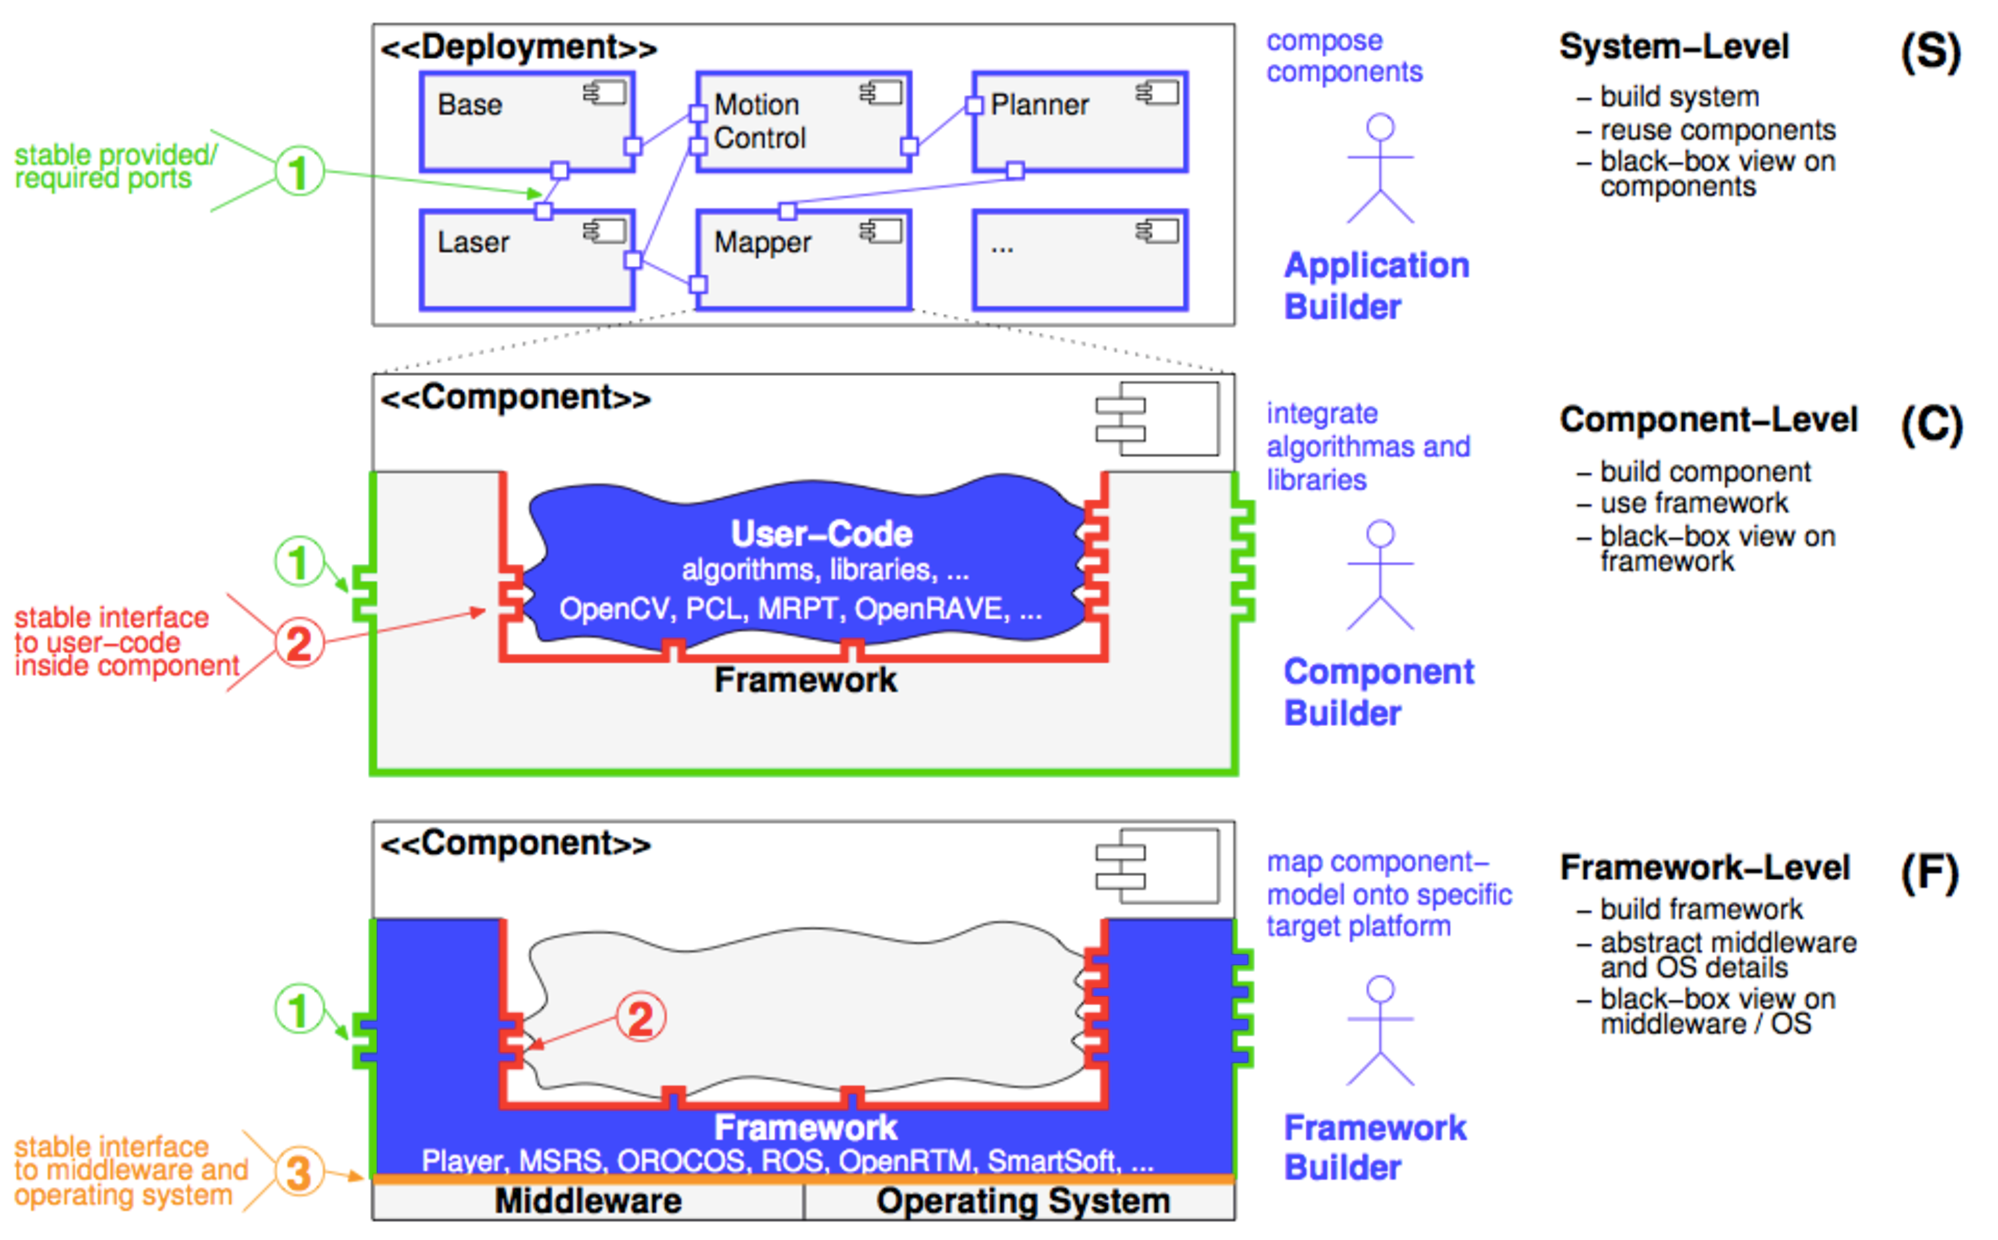
\includegraphics[height=80mm,angle=0]{./figs/levels.pdf}
\end{center}
\caption{The relationship between the robot software system (implemented as a network of components), the robot programming framework (or platform), and the underlying middleware and operating system(s) (from \cite{SchlegelSteckLotz2011}). The existence of stable interfaces is a key attribute of each level.}
\label{fig:levels}       
\end{figure}


\section{Component-based Software Engineering}
%=============================================================
\label{section:componentSE}

\subsection{Background Material}
%------------------------------------------------------------------------------------

The following overview of component-based software engineering focusses on the issues that are particularly important in robot programming. It is based in part on the tutorials by Davide Brugali, Patrizia Scandura, and Azamat Shakhimardanov ``Component-Based Robotic Engineering'' \cite{BrugaliScandurra09,BrugaliShakhamirdanov10}, complemented by material on the BRICS Component Model by Herman Bruyninckx and colleagues \cite{Bruyninckxetal13}, and the paper by Christian Schlegel and colleagues on model-driven software development in robotics \cite{SchlegelSteckLotz2011}, among other sources.


\subsection{Characteristics of Component-Based Software Engineering}
%------------------------------------------------------------------------------------

Targetting the development of reusable software, component-based sofware engineering (CBSE)  complements traditional object-oriented programming by focussing on run-time composition of software rather than link-time composition.  Consequently, it allows different programming languages, operating systems, and possibly communication middleware to be used in a given application.  It harks back to the classic concept of communicating sequential processes (CSP) \cite{Hoare78}, the idea being that components are individually-instantiated processes that communicate  with each other by message-passing. Typically,  component models assume asynchronous message-passing where the communicating component is non-blocking, whereas CSP assumed synchronous communication.   The key idea is that components can act as reusable building blocks and that applications, or system architectures, can be designed by {\em composing} components.   

This gives rise to the two key concerns of component-based models: {\em composability} and {\em compositionality}.  In complex robotics system, integration is difficult.  It is made easier by adopting practices that ``make components more composable and systems more compositional'' \cite{Bruyninckx10}.
	
Thus, {\em composability} is the property of a component to be easily integrated into a larger system, i.e., to be reused under composition, while {\em compositionality} is the property of a system to exhibit predictable performance and behaviour if the performance and behaviour of the components are known.  

Unfortunately, it is not possible to maximize both properties simultaneously because the information hiding characteristic inherent in good component design conflicts with the need for system engineers to optimize system robustness by selecting components with the most resilient and flexible internal design \cite{Bruyninckx10}.


\subsection{Component Granularity and Systems}
%------------------------------------------------------------------------------------

The granularity of {\em components} is larger than that of {\em objects} in object-oriented approaches. Thus, the functionality encapsulated in a component is typically greater than that of an object. Also, components are explicitly intended to be stand-alone reusable pieces of software with well-defined public interfaces.

In general, a component implements a well-encapulated element of robot functionality.  Systems are constructed by connecting components. The connections are made using ports in the components.  As we will see below, this gives rise to the so-called {\em Component-Port-Connector} model.  


\subsection{Component Interfaces}
%------------------------------------------------------------------------------------

In component-based sofware engineering, as in object-oriented programming, the component specification is separated from the component implementation.  A component exposes its functionality through abstract interfaces that hide the underlying implementation.  Thus, the implementation can be altered without affecting any of the systems or other components that use (i.e., interface with) that component.  Components exchange data through their interface.

Interfaces can be classified as either {\em data interfaces} or {\em service interfaces}.  Data interfaces expose state information about the component and typically provide get / set operations for retrieving or setting the values of attributes.   These attributes will typically be specified as abstract properties (in order to keep the implementation hidden).  A service interface is a declaration of the set of functionalities offered by a component on the parameters that are passed to it. 

An interface can be either stateful or stateless.   In a stateful interface, the invocation of an operation changes the component's internal state and the information returned by the operation is computed differently, depending on the component's state.   Thus the behaviour of the exposed operations depends on the history of their previous invocations.  In a stateless interface, the operations's behaviour is always the same and the outcome depends only of the information provided through the parameters, i.e., the data exchanged through the interface. In a stateless interface, a client component has to specify all the information related to its request for the invocation of some operation.  Consequently, a component with a stateless interface can interact with many different clients and client requests since none of them can make any assumptions about the state of the component.

 
\begin{comment}

\section{The BRICS Component Model}
%==============================================================

\begin{figure}[t]
\begin{center}
\includegraphics[height=40mm,angle=0]{./figs/5Cs.pdf}
\end{center}
\caption{The 5 Cs: the core idea is that good component-based engineering practice strives to decouple the design concerns of these five functions (from \cite{Bruyninckxetal13}). }
\label{fig:5Cs}       
\end{figure}

The BRICS Component Model (BCM) provides guidelines, meta-models, and tools for structuring the development of individual components and component-based systems in a framework-nonspecific manner, i.e. at an abstract (meta) level that doesn't refer explicitly to the implementation of the required functionality on a specific robot platform.  

BCM brings together two strands of software engineering: the separation of the so-called 4Cs of communication, computation, configuration and coordination \cite{RadestrockEisenbach96} and Model-Driven Engineering.   

BCM extends the 4Cs to 5Cs by splitting configuration into finer-grained concepts of configuration and composition: see Fig. \ref{fig:5Cs}.  The core idea is that good component-based engineering practice strives to decouple the design and implementation of these five concerns.  We will summarize them briefly.

{\em Computation}  refers to the system's main functionality, i.e. the information processing the component has been designed to perform.
{\em Communication } provides the data required by the computation and takes care of the quality of service of data communication, e.g. timing, bandwith, loss (accuracy), priority, and latency. 
{\em Coordination} refers to the functionality that determines how all the components in a system work together and, thus, how the component or system behaves.  
{\em Configuration} refers to the functional aspects concerned with influencing the behaviour of the computation and communication elements either at start-up or at run-time.
Finally, {\em composition}, the fifth C introduced by Herman Bruyninckx, provides the glue that binds together the other four Cs, each of which is focussed on decoupling functionalty.  In contrast, composition {\em is} concerned with coupling: how the other four Cs interact.  Strictly, the C does not reflect software functionality but is rather a design characteristic that seeks to find a good tradeoff between composability and compositionality. 
\end{comment}

\section{Model-Driven Engineering and the Component-Port-Connector Model}
%==============================================================

\begin{figure}[t]
\begin{center}
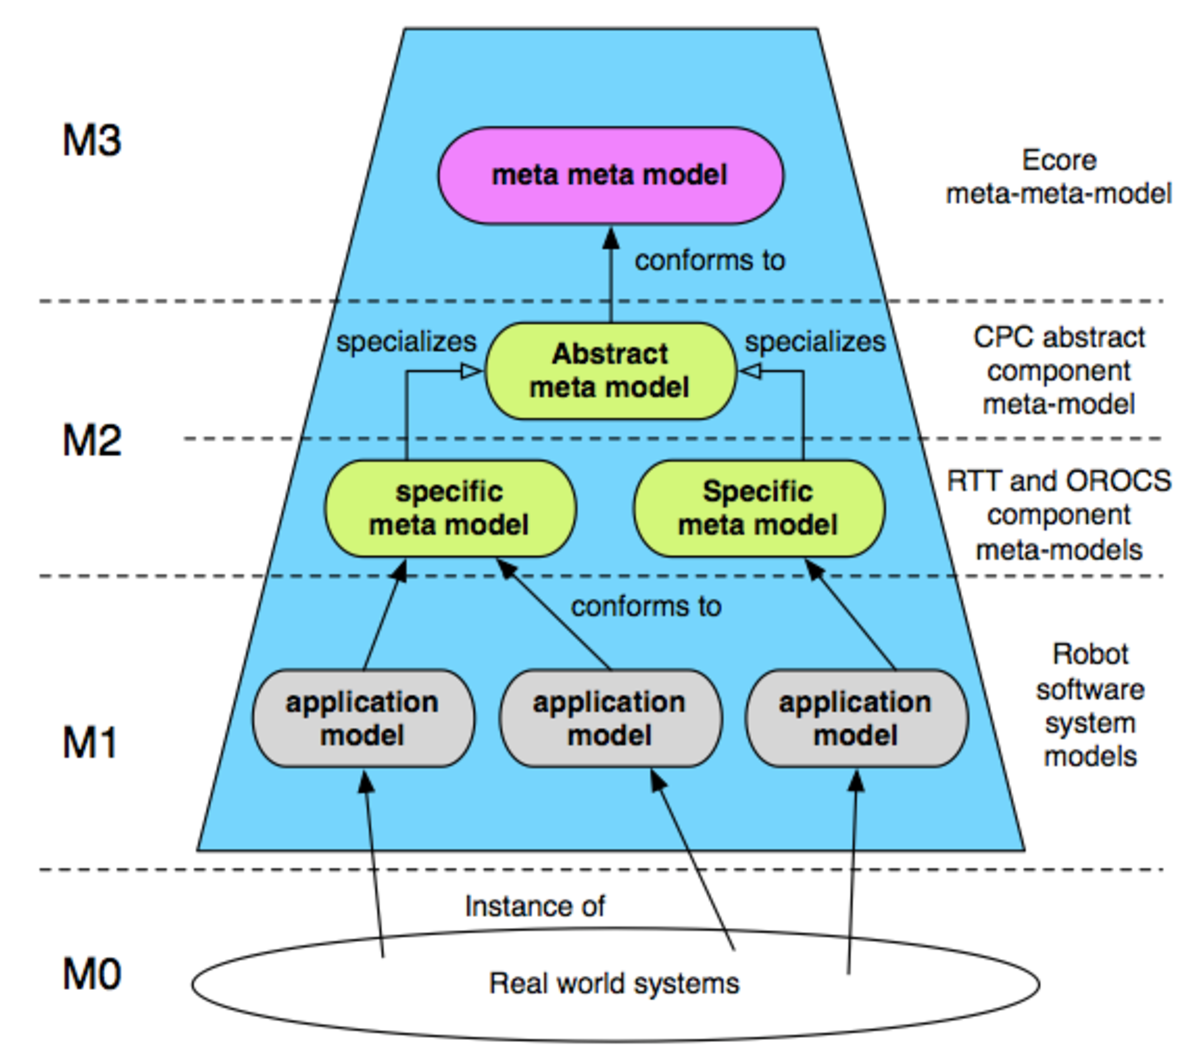
\includegraphics[height=60mm,angle=0]{./figs/OMG.pdf}
\end{center}
\caption{The four levels of abstraction from the OMG \cite{OMG} applied in the BRICS Component Model (from \cite{Bruyninckxetal13}). }
\label{fig:OMG}       
\end{figure}

Model-Driven Engineering (MDE) aims to improve the process of code generation from abstract models that describe a domain.  The Object Management Group (OMG) \cite{OMG}  defines four levels of model abstraction, going from higher to lower levels of domain specificity, i.e., from platform-independent to platform-specific, by adding platform knowledge.  These four levels can be characterized as follows \cite{Bruyninckxetal13} (see also Fig. \ref{fig:OMG}).

\begin{description}
\item[M3] Domain-nonspecific: the highest level of abstraction using a meta-meta-model.
\vspace{-3mm}
\item[M2] Platform-independent representation of a domain: uses a {\em Component-Port-Connector} (CPC) meta-model.
\vspace{-3mm}
\item[M1] Platform-specific model: a concrete model of a specific robotic system but without using a specific programming language.
\vspace{-3mm}
\item[M0] The implementation level of a specific robotic system, with defined software frameworks, libraries, and programming languages.
\end{description}
Of particular interest here is level M2 because  the abstract model, i.e.  the {\em Component-Port-Connector} (CPC) meta-model,  maps directly to the concepts of component-based software engineering.    Figure \ref{fig:CPC} shows a UML diagram representing the CPC meta-model.   The essence of this model is as follows. 
\begin{itemize}
\item An application system has zero or more components and zero or more connectors.  
\item A component has zero or more ports.   
\item A port belongs to one and only one component.  
\item A connector is always between two ports. 
\item Components expose their data and service interfaces on their ports and exchange data over the attached connectors.
\end{itemize}
We are now in a position to identify the guidelines for selecting an appropriate robot programming framework and setting standards for the development component-based software centred on the Component-Port-Connector meta model and model-driven engineering.

\begin{figure}[t]
\begin{center}
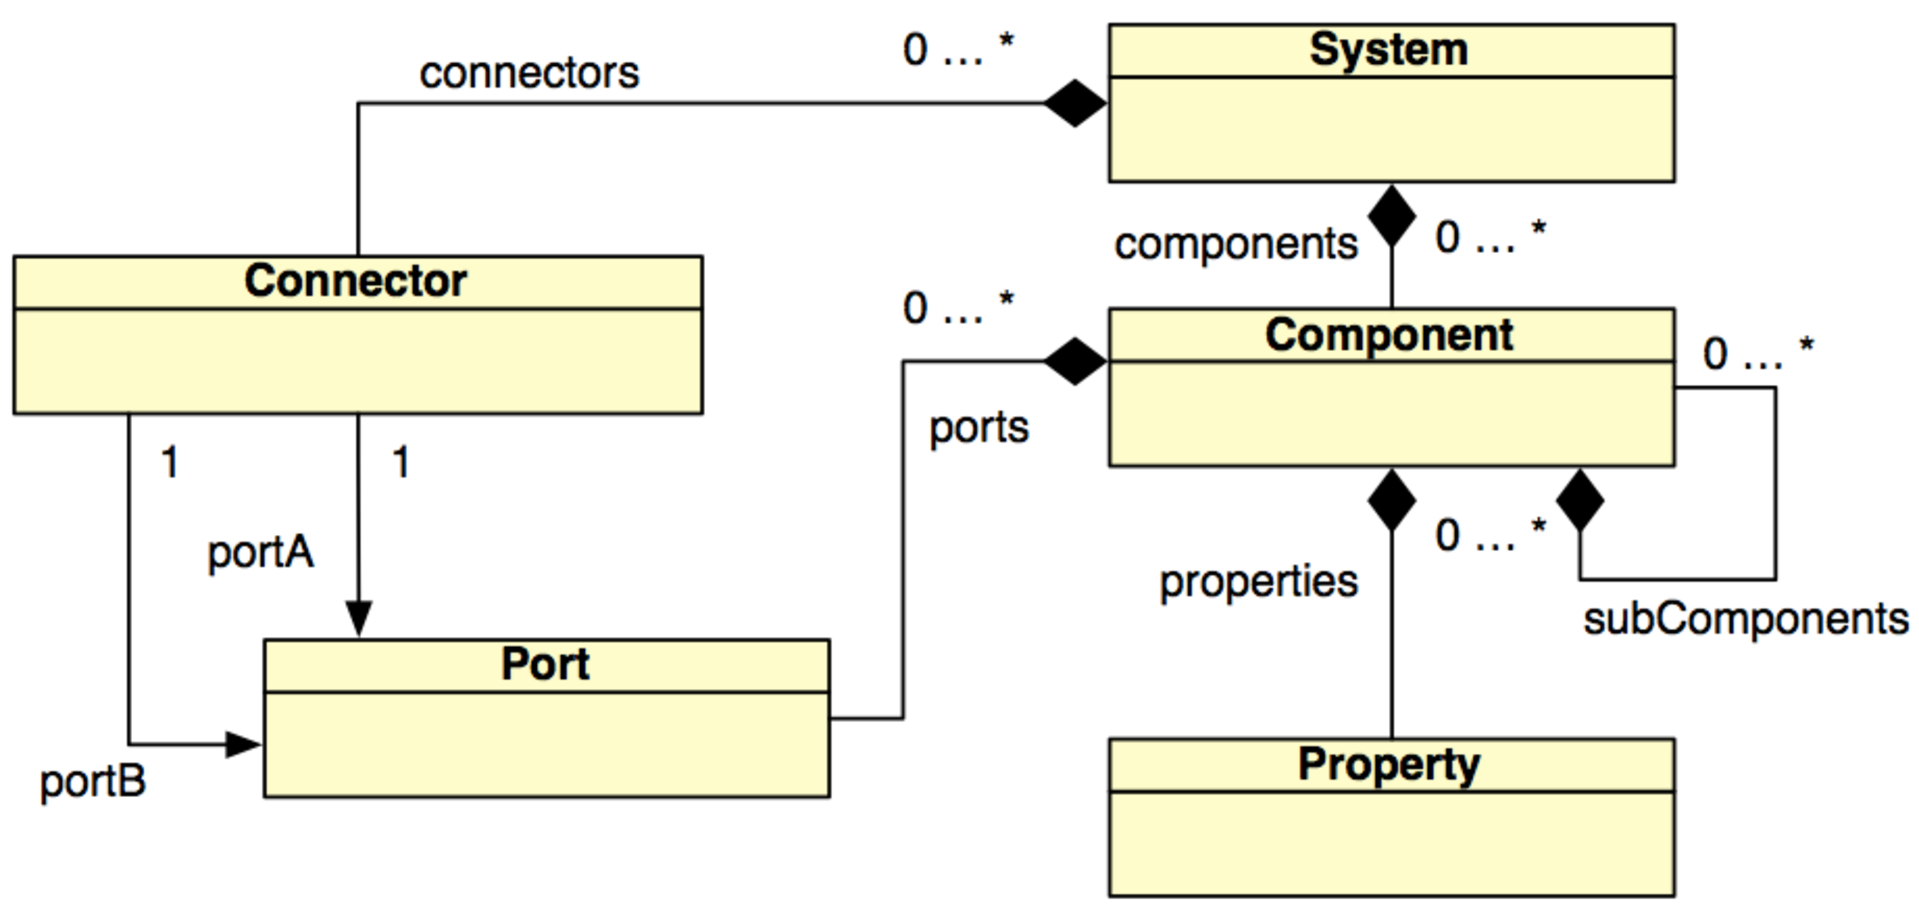
\includegraphics[height=60mm,angle=0]{./figs/CPC.pdf}
\end{center}
\caption{A UML diagram representing the Component-Port-Connector meta-model (from \cite{Bruyninckxetal13}). }
\label{fig:CPC}       
\end{figure}


\newpage

\section{Guidelines}
%==============================================================
\label{section:guidelines}
The principles of CBSE and Level 2 of MDE can be encapsulated in the following guidelines.  These guidelines provide the basis for the choice of robot programming framework and the software development standards in Parts \ref{part:environment} and \ref{part:standards}.

\begin{enumerate}

\item The software engingeering methodology, in general, and the robot programming framework, in particular, should support the {\bf component-port-connector} meta-model,  the principles of component-based software engineering, and the principles of model-driven engineering.

\item The {\bf robot application} should be implemented by identifying the components to be instantiated and specifying the connections between their port interfaces.

\item Each component should encapsulate some  {\bf coarse-grained} robot functionality (i.e. the component should perform some substanial function while maintaining its cohesion and not doing too many disparate things).

\item It should be possible to have {\bf multiple instances} of the same component (this requires a mechanism for uniquely naming each instance of the component and propagating that name to the component's port names).

\item There should be a facility for {\bf external configuration} of the behaviour of the component (this allows the behaviour of individual instances of a component to be customized by the application developer without recourse to the component developer).

\item There should be a facility to allow components to run in {\bf different contexts} (in essence, this means that the robot programming framework should allow the component user to specify the location of the components configuration files and other resources).

\item There should be a facility for {\bf runtime configuration} of the behaviour of the component (this allows users and other components to control the component's processing, if necessary).

\item Configuration should provide explicit {\bf assignment of resources} to the component, where necessary.

\item Components should be able to run and communicate {\bf asynchronously.}

\item It must be possible to run components on a {\bf distributed system} (this requires a mechanism to assign a component to a given compute-server).

\item Components should have {\bf stable interfaces}  (this implies, among other things, that backward compatibility should be assured).

\item The robot programming framework should provide facilities to support {\bf abstract component interfaces} (in effect, this will mean that there is support for high-level communication using ports).

\item There should be flexible communication infrastructure with {\bf multiple transport layer protocols} (this means in effect that the ports can be configured to use different communication protocols, e.g. udp, tcp, and mcast).
 
\item The robot programming framework should provide {\bf graphic user interface tools}  for managing the execution of robot applications. 

\end{enumerate}


\newpage
\part{Software Development Environment}
\label{part:environment}
%#############################################################################
 
\setcounter{section}{0}      % Reset the section numbering in each part
 
In this part, we will identify the six constituents of the CSSR4Africa software development environment:
\begin{enumerate}
\item Programming languages and compilers; \vspace{-3mm}
\item Operating systems; \vspace{-3mm}
\item Robot programming framework; \vspace{-3mm}
\item Make file utilities; \vspace{-3mm}
\item Software libraries \vspace{-3mm}
\item Software repository. \vspace{-0mm}
\end{enumerate}
The  choice of robot programming framework is based directly on the fourteen guidelines set out in the previous section.
Following all guidelines is the ideal. The need to make choices based on existing competences shared by all partners in the consortium may preclude following some guidelines.

A complete set of instructions on how to download and install all the various utilities, libraries, and tools comprising the CSSR4Africa  software development environment will be provided in Deliverable D3.2 Software Installation Manual.  
\begin{comment}
Furthermore, it will provide instructions on how to compile and link an example component and to configure, manage, and run an example robot application comprising a collection of connected components in the CSSR4Africa software respository.   
\end{comment}

\section{Programming languages and compilers}
%=============================================================
CSSR4Africa software should be written in either the C language, the C++ language, or, where necessary, Python.
 

\section{Operating Systems}
%=============================================================
\label{section:os}

Software will be developed for Ubuntu 18.04.


\section{Robot Programming Framework}
%=============================================================
\label{section:framework}

There are many robot programming frameworks. These include ROS \cite{Quigleyetal09}, YARP \cite{MettaFitzpatrickNatale06}, URBI \cite{Baillie05}, and Orca \cite{Soetens06,Brooksetal07}.  All have their respective advantages and disadvantages, as explained in various surveys and comparisons \cite{MakarenkoBrooksKaupp07,Barakovaetal13}.  

Our goal is to select one that will allow the software required to deliver the CSSR4Africa s functionality to be developed efficiently and effectively, bearing in mind constraints of shared partner competences.  As we have already stated, we have adopted the principles of component-based software engineering (CBSE) and fourteen guidelines on the required attributes of a good CBSE framework have been  identified in Part \ref{part:principles}.  

Having considered the  various options, we decided to adopt ROS \cite{ROS} as the framework for CSSR4Africa.  ROS is a popular choice in many projects, despite having been criticized in the context of Component Based Software Engineering for lacking an abstract component model \cite{SchlegelSteckLotz2011}. It has the distinct advantage that both partners in the CSSR4Africa consortium have adopted ROS for their research and teaching in robotics.

In the following, we use the terms {\em component} and {\em node} interchangeably.  In general, we use {\em component} when referring to the  abstract CBSE view of the entity and {\em node} when referring to the ROS implementation of a component. Similarly,  we use the terms {\em port} and {\em  publisher/subscriber/service/action} interchangeably,  the former when referring to the  abstract CBSE view of the entity and latter when referring to the ROS implementation. 
Finally,  we use the terms {\em connector} (CBSE) and {\em topic} (ROS) interchangeably.  Messages are exchanged by publishers and subscribers using ROS topics.  Since communication on ROS topics is non-blocking and open-loop, i.e., a broadcast form of communication between ROS nodes, ROS provides a blocking mechanism, called a {\em service} that provides a two-way communication between nodes. ROS also provides a client-server mechanism, called an {\em action}, that allows status information to be provided by a server node to a client node while the requested operation is being carried out.

We now address the extent to which ROS adheres to the fourteen CBSE guidelines in Part \ref{part:principles}, Section \ref{section:guidelines}.

\subsection{Support for the Component-Port-Connector Meta-Model}
%---------------------------------------------------------------------------------------
ROS supports the {component-port-connector} meta-model as well as the principles of component-based software engineering and the principles of model-driven engineering.  Specifically, a ROS node corresponds to a component and it can have an arbitrary number of publishers and subscribers (ports) communicating using topics (connectors).

\subsection{Robot Applications}
%---------------------------------------------------------------------------------------

ROS supports the implementation of  {robot applications} by identifying the components (nodes) to be instantiated and specifying the connections (topics) between their port interfaces, i.e, using publishers and subscribers (or, possibly, services and actions).  

\subsection{Coarse-grained Functionality}
%---------------------------------------------------------------------------------------

ROS support the encapsulation of  { coarse-grained} robot functionality insofar as the scope of the functionality in a ROS node is under the control of the component developer.  

\subsection{Multiple Instances of Components}
%---------------------------------------------------------------------------------------

ROS supports the instantiation of {\bf multiple instances} of the same component (node). This is achieved using a {\small 
\verb+ __name +} key when running or launching the node.  ROS also allows topic names to be remapped.
 
\subsection{External Configuration}
%---------------------------------------------------------------------------------------

It is accepted best practice in software engineering to ensure that the behaviour of a component can be configured externally, without having to change and recompile the code.  ROS does not have specific tools to effect this, so we will simply adopt the practice of supporting { external configuration} of the behaviour of the component through the use of {\small \verb+.ini+} configuration files, comprising a set of one or more key-value parameters, e.g.,  {\small \verb+threshold <value>+}. This allows the behaviour of individual instances of a component to be customized by the application developer without recourse to the component developer.  It is the responsibility of the component developer to expose all these parameters to the user.   

 
\subsection{Different Contexts}
%---------------------------------------------------------------------------------------

ROS provides a facility to allow components to run in different workspaces.  
 
 
\subsection{Runtime Configuration}
%---------------------------------------------------------------------------------------
\label{section:runtime}

ROS does not provide tools to support runtime configuration. If this is required, it can be effected by periodically invoking the function or method that reads the node configuration file,  re-initializing the parameter values accordingly at runtime.

\subsection{Assignment of Resources}
%---------------------------------------------------------------------------------------

The guidelines state that a CBSE-based robot programming framework should provide explicit {assignment of resources} to the component, where necessary.  
Again,  ROS does not provide tools to support this but such functionality can be accomplished through the configuration file. 

\subsection{Asynchronous Communication} 
%---------------------------------------------------------------------------------------

All ROS nodes run and communicate {asynchronously.}

\subsection{Distributed Computing}
%---------------------------------------------------------------------------------------

ROS supports distributed computing.  It is possible to run components on a network of computers, be it a distributed system, a collection of PCs, or a server farm.  Specifically, YARP allows an application developer (not just a component developer) to assign a component to a given compute-server.  

 

\subsection{Stable Interfaces}
%---------------------------------------------------------------------------------------

This guideline states that components should have {stable interfaces}. This can be ensured by enforcing backward compatability in the development of new code and the modification of legacy code.


\subsection{Abstract Component Interfaces}
%---------------------------------------------------------------------------------------

The robot programming framework should provide facilities to support {abstract component interfaces}.  As noted above, this effectively  means that there is support for high-level communication using ports.  Again, this is the very essence of ROS, for which publishers, subscribers, services, and actions are central to inter-node communication. 

\subsection{Multiple Transport Layer Protocols}
%---------------------------------------------------------------------------------------

ROS supports a flexible communication infrastructure with {multiple transport layer protocols} so that the topics can be configured to use different communication protocols, specifically {\small \verb+TCPROS+} and {\small \verb+UDPROS+}.


\subsection{Graphic User Interface Tools}
%---------------------------------------------------------------------------------------

ROS uses the  {\small \verb+rqt+} metapackage. This is a Qt-based framework for GUI development for ROS.

\section{Make File Utilities}
%=============================================================
\label{section:make}

ROS uses  {\small \verb+catkin+} to manage and build packages, i.e., collections of nodes.   {\small \verb+catkin+} uses  {\small \verb+CMake+}  to provide the build functionality.  


\section{Software Repository}
%=============================================================
\label{section:repository}

The release version of all CSSR4Africa software will be uploaded to the CSSR4Africa repository on GitHub  {\small \verb+https://github.com/cssr4africa/cssr4africa+}.  Software will only be uploaded after it has passed the integration checks set out in Deliverable D3.4 System Integration and Quality Assurance Manual. These checks enforce adherence to the mandatory standards in Appendix \ref{appendix:file_standards} and Appendix \ref{appendix:documentation_standards} of this deliverable.
 

\newpage
\part{Standards}
\label{part:standards}
%#############################################################################
 
\setcounter{section}{0}      % Reset the section numbering in each part

This part of the document defines the project's standards governing the specification, design, documentation, and testing of all software to be developed in work-packages WP4 and WP5.  Particular emphasis is placed on the latter phases of the life cycle --- implementation, testing, and documentation --- because these are particularly important for effective system integration and long-term support by third-party software engineers and system users.  

We distinguish between {\em recommended standards} that reflect desirable practices and {\em mandatory standards} that reflect required practices.  CSSR4Africa component software developers and robot application developers are stongly encouraged to adhere to the desirable practices but these standards do not form part of the checks that will be used to decide whether or not a given component of application can be included in the  CSSR4Africa software repository, as set out in the CSSR4Africa software quality assurance process described in Deliverable D3.4.  On the other hand, the required practices {\em do} form part of the software quality assurance process and {\em a component or application will only be accepted for integration in the release version of the  CSSR4Africa software if it complies with the corresponding mandatory standards.}

In creating the standards set out in this part, we have drawn from several sources.  These include the GNU Coding Standards \cite{Stallman05},
Java Code Conventions \cite{java},
C++ Coding Standard \cite{cpp}, 
EPFL BIRG Coding Standards \cite{epfl}, and Python Enhancement Proposals standards \cite{pep8}.
%%and the Doxygen User Manual \cite{vanHeesch05}.
 

\section{Component and Sub-system Specification}
%=============================================================
\label{section:component_specification}

The  CSSR4Africa project aims to allow researchers and software developers as much freedom as possible in the specification of the components that meet the functional requirements for the culturally sensitive social robotics scenario set out in deliverables D2.2 and D2.3.  Consequently, this phase of the software development life-cycle are subject to following {\em recommended standards}. 

\begin{description}
\item [Requirements]~\\Requirements should be derived from deliverables D2.2 and D2.3 and exemplified by use cases.
\item [Computational model]~\\Any underlying computational model should be clearly documented.
\item [Functional model]~\\A functional specification should be documented, together with a functional decomposition into smaller functional units.  If an object-oriented approach is being used, then the functional model should include a class and class-hierarchy definition.
\item [Data model]~\\The data model should be described with an entity-relationship diagram. A data dictionary should be produced, identifying the input functional, control, system configuration data, output functional, control, system configuration data for each process or thread in the component. If an object-oriented approach is being used, then an object-relationship model should be included.
\item [Process flow model]~\\A process flow model should be produced, e.g., a  data-flow diagram (DFD), identifying data flow, control flow, and persistent data sources and sinks.
\item [Behavioural model]~\\A behavioural model should be produced, e.g., a state transition diagram. If an object-oriented approach is being used, then an object-behaviour model should be included.
\end{description} 

 

\section{Component Design}
%=============================================================
\label{section:component_design}

The principles of good design have already been addressed at length in Part \ref{part:principles}, in general, and in the guidelines set out in Part \ref{part:principles}, Section \ref{section:guidelines}, in particular.  We consider these guidelines to be a set of {\em recommended standards} for component design and we will not repeat them here.  However, it is important to note that these guidelines give rise to several essential practices --- and mandatory standards --- in component implementation.  We return to these in the next section. 
 

\section{Component Implementation}
%=============================================================
\label{section:component_implementation}

Some implementation standards are mandatory, others are recommended.  The mandatory standards for implementation of components  form part of the software quality assurance process and the component  will only be accepted for integration in the release version of the CSSR4Africa  software if it complies with these standards.  
\\~\\
\noindent The {\em mandatory} implementation standards include the following.   

\begin{enumerate}
\item Mandatory standards for file names and  file organization (Appendix \ref{appendix:file_standards}).
\item Mandatory standards for internal source code documentation  (Appendix \ref{appendix:documentation_standards}).
\end{enumerate}


\noindent The {\em recommended} implementation standards include the following.  
\begin{enumerate}
\item Recommended standards for programming style (Appendix \ref{appendix:programming_style_standards}).
\item Recommended standards on programming practice (Appendix \ref{appendix:programming_practice_standards}).
\end{enumerate}

\begin{comment}
To make them easier to follow, all these standards make reference to a ROS implementation of an example component (i.e., a ROS node) which will be made available on the  CSSR4Africa GitHub repository along with a sample application.   Support documentation will be provided on the CSSR4Africa  wiki.
 \end{comment}
 
\section{Testing}
%=============================================================
\label{section:testing}

CSSR4Africa  software will be subject to a spectrum of test procedures, including black-box unit tests, system tests, and regression tests.

\subsection{Black-box Unit Tests}
\label{section:black_box_tests}

Black-box testing is a testing strategy that checks the behaviour of a software unit --- in this case a component --- without being concerned with what is going on inside the unit; hence the term ``black-box''.   Typically, it does this by providing a representative sample of input data (both valid and invalid), by describing the expected results, and then by running the component against this test data to see whether or not the expected results are achieved. 
\blank
~
\blank
Component software developers must provide up to three unit tests with every component submitted for integration into the CSSR4Africa  release.     These tests comprises  a launch file and a test description. Both should be located in the {\small \verb+launch+} directory (see Appendix A). The three tests are  either the physical robot, the simulator, or a driver/stub test harness.
\blank
~
\blank
The launch files should launch the node being tested and, depending on which test is being run,  the physical robot, the simulator, or a driver node to source (publish) test data, and a stub node to sink  (subscribe to) the output of the node being tested.   
\blank
~
\blank
The launch files  should be named after the component but with the filename extension {\small \verb+.launch+}.\\ For example: {\small \verb+exampleComponentLaunchRobot.launch+}, \\{\small \verb+exampleComponentLaunchSimulator.launch+}, and\\ {\small \verb+exampleComponentLaunchTestHarness.launch+}.  
\blank
~
\blank
Instructions on how to run the tests should be included in a {\small \verb+README.md+} file, also located in the  {\small \verb+launch+}  directory (see Appendix \ref{appendix:file_standards}). 
In general, these instructions should describe the nature of the test data and the expected results, and it should explain how these results validate the expected behaviour of the component.    


\subsection{System  Tests}
\label{section:system_tests}
 
A set of system tests will launch a subset of the components (nodes) in the system architecture to check that they provide  the required functionality. The final two system tests will lauch the entire system and run the two user interaction scenarios.

\subsection{Regression Tests}
\label{section:regression_tests}
Regression testing refers to the practice of re-running all  tests periodically to ensure that no  unintentional changes has been introduced during the ongoing development of the CSSR4Africa software release.   These tests check for backward compatability, ensuring that what used to work in the past still works now.    Regression tests will be carried out on all software in the CSSR4Africa release every three months.

 


\section{Documentation}
%=============================================================
\label{section:documentation_standards}

The primary vehicle for documentation will be the CSSR4Africa wiki. It will have sections dealing with the following five issues.

\begin{enumerate}
\item Software installation guide.
\item Software development guide (based on this deliverable, i.e., Deliverable D3.3).
\item Software integration guide (based on Deliverable D3.4).
\item Component reference manual.
\end{enumerate}
The software installation guide will provide a step-by-step guide to downloading, installing, and checking the software required to develop CSSR4Africa software  and run CSSR4Africa robot applications.   It will derived from  Deliverable D3.3.
\blank
~
\blank
The software development guide will be derived directly from the relevant sections of this deliverable (D3.2), addressing the development of component software and robot applications.   
\begin{comment}
It will include a detailed step-by-step walkthough of the design and implementation of the example  component {\small \verb+exampleComponent+} used throughout  this deliverable and the development of an application to use it.
\end{comment}
\blank
~
\blank
The software integration guide will describe the procedures for unit testing of individual components and submitting them for integration.  This guide  will be derived from Part \ref{part:standards}, Section \ref{section:testing} of this deliverable, from Deliverable D3.4, and augmented with more detailed instructions whereever they are needed.
\blank
~
\blank
The component reference manual will be derived from the contents of the node {\small \verb+README.md+} file (see Appendix \ref{appendix:file_standards}, Section A.3) and the first documentation comment in the node application file (see Appendix \ref{appendix:documentation_standards}, Section B.2).
\begin{comment}
mainly from the Doxygen documentation comments in the header file of each component; see Appendix \ref{appendix:documentation_standards}, Section \ref{section:documentation_comments} for details of the information that is captured in this documentation.
\end{comment}
\blank
~
\blank
For easy reference, the wiki  will also include copies of the standards described in this deliverable.
\begin{enumerate}
\item Mandatory Standards for File Organization
\item Mandatory Standards for Internal Documentation
%%\item Mandatory Standards for Component Functionality
%%\item Mandatory Standards for Testing
\item Recommended Standards for Programming Style
\item Recommended Standards for Programming Practice
\end{enumerate}
The mandatory standards are contained in Appendices \ref{appendix:file_standards} and
\ref{appendix:documentation_standards}, 
(File Organization and Internal Documentation, respectively), as well as Section \ref{section:testing} on Testing.
The recommended standards are contained in Appendices \ref{appendix:programming_style_standards}  and
\ref{appendix:programming_practice_standards}    (Programming Style and Programming Practice, respectively).

\pagebreak


\begin{appendices}
%###############################################################################

%===============================================================
\section{Mandatory Standards for  File Organization}
%===============================================================
\label{appendix:file_standards}  




\subsection{Directory Structure}
%-------------------------------------------------------------------------------------
\label{section:directory_structure}

CSSR4Africa software adheres to the standard ROS directory structure for a ROS workspace.
There are, in fact, two CSSR4Africa ROS workspaces, one for the physical Pepper robot ({\small \verb+pepper_rob_ws+}) and one for the simulator ({\small \verb+pepper_sim_ws+}).  The directory structure is identical, as shown in Fig. \ref{fig:directory_structure} for the {\small \verb+pepper_rob_ws+} workspace. 

\begin{figure}[th]
\begin{multicols}{3}

~~~~~~~~~~~~~~~~~~~~~

\vspace{20cm}

\columnbreak

{\small 
\dirtree{%
.1 workspace.
.2 pepper\_rob\_ws.
.3 build.
.3 devel.
.3 src.
.4 cssr4africa.
.5 cssr\_system.
%%.5 animate\_behavior.
%%.5 attention.
%%.5 gesture\_speech\_navigation.
%%.5 interaction\_events.
%%.5 interaction\_manager.
.5 pepper\_interface\_tests.
%%.5 sensing.
.5 system\_tests.
%%.5 user\_interface.
.5 unit\_tests.
.4 naoqi\_dcm\_driver.
.4 naoqi\_driver.
.4 pepper\_dcm\_robot.
.4 pepper\_moveit\_config.
.4 pepper\_robot.
.4 pepper\_virtual.
}
}


\columnbreak

~~~~~~~~~~~~~~~~~~~~~

\end{multicols}
\caption{Directory structure for the CSSR4Africa software repository.}
\label{fig:directory_structure}       
\end{figure}

\noindent The {\small \verb+cssr4africa+} directory is a ROS metapackage which collects together the ten ROS packages that make up the CSSR4Africa system. Six of these are CSSR4Africa system architecture packages and four are auxilliary packages, as shown in Table \ref{table:packages}.
\blank
~
\blank
Each package has a similar directory structure. For example, see the directory structure for \\
{\small \verb+pepper_interface_tests+} in Fig. \ref{fig:tests}.  In this case, there are two ROS nodes: {\small \verb+actuatorTest+} and {\small \verb+sensorTest+}.  Eventually, the six system architecture packages will be populated with the components (nodes) specified in the CSSR4Africa work plan, augmented by any other components that are identified when designing the system architecture in Task 3.1.


\begin{table}[thb]
\begin{center}
\begin{tabular}{|l l|}
\hline  \hline
\multicolumn{2}{|c|}{ {\bf System Architecture Packages}} \\
\hline
Architecture Subsystem                & Package Name \\
\hline
Animate Behaviour 	                     & {\small \verb+cssr_system+} \\
Attention	                                     & {\small \verb+cssr_system+} \\
Gesture, Speech, \& Navigation     & {\small \verb+cssr_system+} \\
Detection of Interaction Events     & {\small \verb+cssr_system+}  \\
Interaction Manager                     & {\small \verb+cssr_system+} \\
Sensing \& Analysis                     &  {\small \verb+cssr_system+} \\
\hline 
\hline
\multicolumn{2}{|c|}{{\bf Test Packages}}  \\
\hline
Test Type                & Package Name \\
\hline
Sensor and Actuator Tests         & {\small \verb+pepper_interface_tests+} \\
System Tests                             & {\small \verb+system_tests+} \\
%%User Interface	                           & {\small \verb+user_interface+} \\
Unit Tests                                  & {\small \verb+unit_tests+} \\
\hline \hline
\end{tabular}
\end{center}
\caption{The ROS packages that comprise the CSSR4Africa software system.}
\label{table:packages}
\end{table}


\begin{figure}[thb]
\begin{multicols}{3}

~~~~~~~~~~~~~~~~~~~~~

\vspace{20cm}

\columnbreak

{\small 
\dirtree{%
.1 pepper\_interface\_tests.
.2 config.
.3 actuatorTestConfiguration.ini.
.3 sensorTestConfiguration.ini.
.2 data.
.3 pepperTopics.dat.
.3 simulatorTopics.dat.
.3 sensorTestOutput.dat.
.3 actuatorTestInput.dat.
.3 sensorTestInput.dat.
.2 include.
.3 pepper\_interface\_tests.
.4 actuatorTestInterface.h.
.4 sensorTestInterface.h.
.2 launch.
.3 actuatorTestLaunchRobot.launch.
.3 sensorTestLaunchRobot.launch.
.3 interfaceTestLaunchSimulator.launch.
.2 src.
.3 actuatorTestApplication.cpp.
.3 actuatorTestImplementation.cpp.
.3 sensorTestApplication.cpp.
.3 sensorTestImplementation.cpp.
.2 README.md.
.2 CMakeLists.txt.
.2 package.xml.
}
}
\columnbreak


~~~~~~~~~~~~~~~~~~~~~

\end{multicols}
\cprotect\caption{Directory structure for the  {\small \verb+pepper_interface_tests+} package. There are two nodes: {\small \verb+actuatorTest+} and {\small \verb+sensorTest+}.  }
\label{fig:tests}       
\end{figure}

%\newpage

\newpage

\subsection{Filename Roots and Extensions}
%-------------------------------------------------------------------------------------

\subsubsection{C/C++Programming Language}

All files should have the same root, reflecting computational purpose of the component, 
\blank
e.g.,  {\small \verb+exampleComponent+}.
Other filenames are derived from this by appending the appropriate string to denote the files function. For example, an {\small \verb+exampleComponent+} node would have the following files. \vspace{-2mm} These are explained in the following sections.
\begin{itemize}
\item {\small \verb+exampleComponentApplication+}. \vspace{-2mm}
\item {\small \verb+exampleComponentImplementation+}. \vspace{-2mm}
\item {\small \verb+exampleComponentInterface+}. \vspace{-2mm}
\item {\small \verb+exampleComponentConfiguration+}. \vspace{-2mm}
\item {\small \verb+exampleComponentInput+}. \vspace{-2mm}
\item {\small \verb+exampleComponentOutput+}. \vspace{-2mm}
\item {\small \verb+exampleComponentDriver+}. \vspace{-2mm}
\item {\small \verb+exampleComponentStub+}. \vspace{-2mm}
\item {\small \verb+exampleComponentLaunchRobot+}. \vspace{-2mm}
\item {\small \verb+exampleComponentLaunchSimulator+}. \vspace{-2mm}
\item {\small \verb+exampleComponentLaunchTestHarness+}. \vspace{-2mm}
\end{itemize}
\blank
 Source code files for C and C++ should use a  {\small \verb+.c+} and {\small \verb+.cpp+} extension, respectively.
\blank
~
\blank
Header files should have a {\small \verb+.h+} extension in both cases.

\subsubsection{Python Programming Language}
All files should have the same root, reflecting computational purpose of the component, 
\blank
e.g.,  {\small \verb+example_component+}.
Other filenames are derived from this by appending the appropriate string to denote the files function. For example, an {\small \verb+example_component+} node would have the following files. \vspace{-2mm} These are explained in the following sections.
\begin{itemize}
\item {\small \verb+example_component_application+}. \vspace{-2mm}
\item {\small \verb+example_component_implementation+}. \vspace{-2mm}
\item {\small \verb+example_component_interface+}. \vspace{-2mm}
\item {\small \verb+example_component_configuration+}. \vspace{-2mm}
\item {\small \verb+example_component_input+}. \vspace{-2mm}
\item {\small \verb+example_component_output+}. \vspace{-2mm}
\item {\small \verb+example_component_driver+}. \vspace{-2mm}
\item {\small \verb+example_component_stub+}. \vspace{-2mm}
\item {\small \verb+example_component_launch_robot+}. \vspace{-2mm}
\item {\small \verb+example_component_launch_simulator+}. \vspace{-2mm}
\item {\small \verb+example_component_launch_test_harness+}. \vspace{-2mm}
\end{itemize}
\blank
 {\noindent Source code files for python should use a  {\small \verb+.py+} extension.}
~
\blank
~
\blank
~
Header files should have a {\small \verb+.h+} extension.
 
 \newpage
\subsection{File Organization}
%-------------------------------------------------------------------------------------
 \label{section:file_organization}

\subsubsection{Source Files}

The preferred practice for software that supports encapsulation and data hiding, as, arguably, all software should, is for there to be three types of source file, as follows. 
\begin{enumerate}
\item Application files. \vspace{-2mm}
\item Implementation files. \vspace{-2mm}
\item Interface files.\vspace{-2mm}
\end{enumerate}
The basis for this approach is that application developers should not need to know about the implementation of the classes, methods, functions, and data structures that they are using.  This allows the implementation to be changed without affecting the application.
\blank
~
\blank
Thus, the {\em application file}, e.g., {\small \verb+exampleComponentApplication.cpp+}  or { \\{\small \verb+example_component_application.py+}},  contains the {\small \verb+main()+} function and the code that instantiates the classes, methods, functions, and data structures to effect the required functionality for the application in question.
\blank
~
\blank
The {\em implementation file}, e.g., {\small \verb+exampleComponentImplementation.cpp+} {or \\ {\small \verb+example_component_implementation.py+}}, contains the definitions of the classes, methods, functions, and data structures that implement the algorithms used in the implementation. Ideally, to facilitate reuse, the  implementation should be quite general.
\blank
~
\blank
The {\em interface file}, e.g., {\small \verb+exampleComponentInterface.h+}, contains the declarations required to use the classes, methods, functions, and data structures  that implement the solution to this problem. Thus, the interface file must furnish all the necessary information to use these classes, methods, functions, and data structures.
\blank
~
\blank
The application and implementation files {\small \verb+#include+} the {\small \verb+exampleComponentInterface.h+} file.
\blank
~
\blank
In the particular case of  CSSR4Africa software, the application file contains the code that instantiates the ROS node along with any required classes, reads the {\small \verb+.ini+} configuration file to set the parameter values that govern the behaviour of the node, and calls the functions (C) or invokes the methods (C++ or Python) that provide the required functionality.
\blank
~
\blank
The implementation file contains the source code for the implementation of each class method (C++ or Python) or the source code of each function (C). General purpose functions might eventually be placed in a library.  
\blank
~
\blank
The interface file  is a header file with the class declarations and method  declarations but no method implementations (C++) or  the function  implementations (C). 
\blank
~
\blank
The application and implementation files should be placed in the {\small \verb+src+}  directory, and the interface file in the node subdirectory in the {\small \verb+include+} directory; see Fig. \ref{fig:tests}. Source files for any driver or stub nodes associated with the unit test , e.g., {\small \verb+exampleComponentDriver.cpp+} or \\ {\small \verb+example_component_driver.py+}, and {\small \verb+exampleComponentStub.cpp+}  or \\{\small \verb+example_component_stub.py+}, should also be placed in the {\small \verb+src+}  directory.
\blank
~
\blank
Figure \ref{fig:c++directory}  shows the directory structure for software written in C++ while Figure \ref{fig:pythondirectory}  the directory structure for software written in Python. It shows the package (\verb+example_package+) which is similar to the \verb+cssr_system+ or \verb+unit_tests+ package, and the node (\verb+exampleComponent+ or \verb+example_component+) which is similar to the nodes specified in Table \ref{table:packages} in Deliverable D3.1 System Architecture.

\newpage

\begin{figure}[thb]
 
\begin{multicols}{3}

~~~~~~~~~~~~~~~~~~~~~

\vspace{20cm}

\columnbreak

{\small 
\dirtree{%
.1 example\_package.
.2 exampleComponent.
.3 config.
.4 exampleComponentConfiguration.ini.
.4 exampleComponentInput.ini.
.3 data.
.4 pepperTopics.dat.
.4 simulatorTopics.dat.
.4 exampleComponentOutput.dat.
.4 exampleComponentInput.dat.
.3 include.
.4 example\_package.
.5 exampleComponentInterface.h.
.3 launch.
.4 exampleComponentLaunchRobot.launch.
.4 exampleComponentLaunchSimulator.launch.
.3 msg.
.4 msgFile.msg.
.3 src.
.4 exampleComponentApplication.cpp.
.4 exampleComponentImplementation.cpp.
.3 srv.
.4 srvFile.srv.
.3 README.md.
.3 CMakeLists.txt.
.2 package.xml.
.2 README.md.
.2 CMakeLists.txt.
}
}
\columnbreak


~~~~~~~~~~~~~~~~~~~~~

\end{multicols}
\cprotect\caption{Directory structure for the  software written in C++ }
\label{fig:c++directory}       

\end{figure}


\newpage

\begin{figure}[thb]
 
\begin{multicols}{3}

~~~~~~~~~~~~~~~~~~~~~

\vspace{20cm}

\columnbreak

{\small 
\dirtree{%
.1 example\_package.
.2 example\_component.
.3 config.
.4 example\_component\_configuration.ini.
.4 example\_component\_input.ini.
.3 data.
.4 pepper\_topics.dat.
.4 simulator\_topics.dat.
.4 example\_component\_output.dat.
.4 example\_component\_input.dat.
.3 launch.
.4 example\_component\_launch\_robot.launch.
.4 example\_component\_launch\_simulator.launch.
.3 msg.
.4 msg\_file.msg.
.3 src.
.4 example\_component\_application.py.
.4 example\_component\_implementation.py.
.3 srv.
.4 srv\_file.srv.
.3 models.
.4 example\_component\_model.
.3 README.md.
.3 CMakeLists.txt.
.2 package.xml.
.2 README.md.
.2 CMakeLists.txt.
}
}

\columnbreak
~~~~~~~~~~~~~~~~~~~~~
\end{multicols}
\cprotect\caption{Directory structure for the  software written in Python}
\label{fig:pythondirectory}       

\end{figure}


\subsubsection{Launch Files}
\label{section:launch_files}

The {\small \verb+launch+} directory should contain up to three launch files, one for use with the physical robot, one for use with the simulator, and one for use with the driver and stub test harness.  They should be named after the component but with a {\small \verb+.launch+} filename extension. For example \\
{\small \verb+exampleComponentLaunchRobot.launch+},
 {\small \verb+exampleComponentLaunchSimulator.launch+},   \\
and {\small \verb+exampleComponentLaunchTestHarness.launch+}, or\\
{\small \verb+example_component_launch_robot.launch+}, \\
 {\small \verb+example_component_launch_simulator.launch+},   \\
and {\small \verb+example_component_launch_test_harness.launch+}.  

These launch files are in effect the component unit tests and will be used to validate that the component works correctly and will be used to test the component when it is being submitted for integration, and subsequently transferred to the   {\small \verb+unit_tests+} package.  As such, they should instantiate any necessary driver or stub nodes, the simulator, or the Pepper robot drivers.   Instructions on how to run the tests should be included in a {\small \verb+README.md+} file in the same directory.

\newpage
\subsubsection{Configuration Files}
Each component must have an associated configuration file, named after the component, \\
e.g.,  {\small \verb+exampleComponentConfiguration.ini+}  for C++, and \\
{\small \verb+example_component_configuration.ini+}  for Python.  It is placed in the  {\small \verb+config+}  directory.
\blank
~
\blank
The configuration file contains the key-value pairs that set the component parameters.  For readability, each key-value pair should be written on a separate line.


\subsubsection{Data Files}

A component may have an associated input or output data files. In general, these should be named after the component, appended with either {\small \verb+Input+} or  {\small \verb+Output+}, and have either a  {\small \verb+.dat+}  or {\small \verb+.xml+}   filename extension, 
e.g.,  {\small \verb+exampleComponentInput.dat+} for C++, and 
{\small \verb+example_component_input.dat+}  for Python. However, other filenames are allowable, provided they have a {\small \verb+.dat+}  or {\small \verb+.xml+}=  filename extension.  These files are placed in the  {\small \verb+data+}  directory.

\subsubsection{Other Files}

Three other files are stored in the package directory, as follows.
\begin{enumerate}
\item {\small \verb+README.md+} \vspace{-2mm}
\item {\small \verb+CMakeLists.txt+} \vspace{-2mm}
\item {\small \verb+package.xml+} 
\end{enumerate}
The {\small \verb+README.md+}  file  provides information about the package in a Markdown markup language. It should  describe each node in the package and explain how to use them.   The content will be based on the documentation provided with  nodes when they are submitted for integration and inclusion in the release of CSSR4Africa repository on GitHub. 
\blank
~
\blank
The {\small \verb+CMakeLists.txt+}  file contains the build directives for each node in the package.  It will be based on the CMakeLists.txt that are  provided with  nodes when they are submitted for integration and inclusion in the release of CSSR4Africa repository on GitHub. 
\blank
~
\blank
The  {\small \verb+package.xml+} file contains the package {\em manifest}. This defines details about the package, such as the name, version, maintainer, and dependencies.


\newpage 


\section{Mandatory Standards for Internal Source Code Documentation}
%===============================================================
\label{appendix:documentation_standards}  
  
 \subsection{General Guidelines}
%---------------------------------------------------------------------------------------

Two types of comments are required:  documentation comments and  implementation comments.   Documentation comments describe the functionality of a component from an implementation-free perspective. 
Together with the contents of  the node {\small \verb+README.md+}  file, they will be used to create the documentation in the component reference manual on the CSSR4Africa wiki.  They are intended to be read by developers who won't necessarily have the source code at hand.  Thus, documentation comments help a developer understand how to use the component through its application programming interface (API), e.g, the ROS topics, services, and actions it uses to communicate with other ROS nodes, rather than understand its implementation. Implementation comments explain or clarify some aspect of the code. They should be used to give overviews of code and provide additional information that is not readily available in the code itself. Comments should contain only information that is relevant to reading and understanding the program.   
\blank
~
\blank
Documentation comments are delimited by {\small \verb+/* ... */+} in \texttt{C++} and {\small \verb+""" ... """+  in \texttt{Python}}.
\blank
~
\blank
Implementation comments are delimited by {\small \verb+/* ... */+} and {\small \verb+//+} in \texttt{C++} and {\small \verb+#+}  in \texttt{Python}.
\blank
~
\blank
All comments should be written in English.


\subsection{Documentation Comments}
%---------------------------------------------------------------------------------------
 \label{section:documentation_comments}


{\bf The First Documentation Comment} \\
All C++ source files must begin with a documentation comment that identifies the file being documented, and gives a copyright notice, as follows.  
%\blank
{\small
\begin{verbatim}
/* <filename> <one line to identify the nature of the file>
 *
 * Author:
 * Date:
 * Version:
 * 
 * Copyright (C) 2023 CSSR4Africa Consortium
 * 
 * This project is funded by the African Engineering and Technology Network (Afretec) 
 * Inclusive Digital Transformation Research Grant Programme. 
 *
 * Website: www.cssr4africa.org
 *
 * This program comes with ABSOLUTELY NO WARRANTY.
 */
\end{verbatim}
}

\newpage
\noindent All Python source files must begin with a documentation comment that identifies the file being documented, and gives a copyright notice, as follows.  
%\blank
{\small
\begin{verbatim}
""" <filename> <one line to identify the nature of the file>
 
     Author:
     Date:
     Version:
 
     Copyright (C) 2023 CSSR4Africa Consortium
 
     This project is funded by the African Engineering and Technology Network (Afretec) 
     Inclusive Digital Transformation Research Grant Programme. 
  
     Website: www.cssr4africa.org
 
 This program comes with ABSOLUTELY NO WARRANTY.

 """
\end{verbatim}
}


\newpage 
\noindent The {\small \verb+<componentName>Application.cpp+} file must also contain additional information, documenting the component API. The following is a list of the mandatory sections for which documentation comments must be provided.  

{\small
\begin{verbatim}
/* <componentName>Application.cpp <one line to identify the nature of the file>
 *
 * <detailed functional description>
 *
 ...
 * Libraries
 ...
 * Parameters 
 *
 * Command-line Parameters
 ...
 * Configuration File Parameters
 ... 
 * Subscribed Topics and Message Types
 ...                     
 * Published Topics and Message Types
 ...
 * Input Data Files
 *
 * <componentName>Input.dat
 ...
 * Output Data Files
 *
 * <componentName>Output.dat
 ...
 * Configuration Files
 *
 * <componentName>Configuration.ini 
 ... 
 * Example Instantiation of the Module
 *
 * rosrun <componentName> __name:=<alternativeComponentName> ...
 ...
 * 
 * Author:  <name of author>, <author institute>
 * Email:   <preferred email address>
 * Date:
 * Version:
 *
 */
\end{verbatim}
}

\newpage
 
\noindent The {\small \verb+<component_name>_application.py+} file must also contain additional information, documenting the component API. The following is a list of the mandatory sections for which documentation comments must be provided.  
 
{\small
\begin{verbatim}
""" <component_name>_application.py <one line to identify the nature of the file>
    <detailed functional description>

 ...
    Libraries
 ...
    Parameters 

    Command-line Parameters
 ...
    Configuration File Parameters
 ... 
    Subscribed Topics and Message Types
 ...                     
    Published Topics and Message Types
 ...
    Input Data Files

    <component_name>_input.dat
 ...
    Output Data Files

    <component_name>_output.dat
 ...
    Configuration Files

    <component_name>_configuration.ini 
 ... 
    Example Instantiation of the Module

    rosrun <component_name>_application.py __name:=<alternative_component_name> ...
 ...

    Author:  <name of author>, <author institute>
    Email:   <preferred email address>
    Date:
    Version:

 """
\end{verbatim}

}

\subsection{Implementation Comments}
%---------------------------------------------------------------------------------------

Programs can have four styles of implementation comments: block, single-line, trailing, 
and end-of-line.
\blank
~
\blank
{\bf Block Comments}\\
Block comments are used to provide descriptions of files, methods, data structures, and
algorithms.  Block comments may be used at the beginning of each file and before each
method.  They can also be used in other places, such as within methods.  
Block comments inside a function or method should be indented to the same level as the 
code they describe.
\blank
~
\blank
In C++, a block comment should be preceded by a blank line to set it apart from the rest of the code.
{\small
\begin{verbatim}
   /*
    * Here is a block comment. 
    */
\end{verbatim}
}
\blank
~
\blank
In, Python, block comments generally apply to some (or all) code that follows them, and are indented to the same level as that code. Each line of a block comment starts with a \verb+#+ and a single space (unless it is indented text inside the comment).
\blank
~
\blank
Paragraphs inside a block comment are separated by a line containing a single \verb+#+.
{\small
\begin{verbatim}
   #
   # Here is a block comment. 
   #
\end{verbatim}
}
\blank
~
\blank
{\bf Single-Line Comments}
~
\blank
Short comments can appear on a single line indented to the level of the code that follows.
If a comment can't be written in a single line, it should follow the block comment format.

In C++ ,
{\small
\begin{verbatim}
   if (condition) {

      /* Handle the condition. */

      ...
   }
\end{verbatim}
}

In Python , 
{\small
\begin{verbatim}
   if condition:

      """ Handle the condition. """

      ...
   
\end{verbatim}
}


\blank
~
\blank
{\bf Trailing Comments}
~
\blank
Very short comments can appear on the same line as the code they describe, 
but should be shifted far enough to separate them from the statements.
If more than one short comment appears in a segment of code, they should all
be indented to the same level.

\newpage
\noindent
In C++,
{\small
\begin{verbatim}
   if (a == b) {
      return TRUE;                 /* special case */
   }
   else {
      return general_answer(a);    /* only works if a != b */
   }
\end{verbatim}
}

\noindent
In Python, trailing comments should be separated by at least two spaces from the statement. They should start with a \# and a single space.
{\small
\begin{verbatim}
   if a == b: 
      return True                 # special case

   else:
      return general_answer(a)    # only works if a != b 

\end{verbatim}
}


~
\blank
{\bf End-Of-Line Comments}
~
\blank
In C++, the {\small \verb+//+} comment delimiter can comment out a complete line or only a partial line.
It shouldn't be used on consecutive multiple lines for text comments.  However, it can be used
in consecutive multiple lines for commenting out sections of code.  Examples of all three styles
follow.

{\small
\begin{verbatim}
   if (foo > 1) {

      // look left
      ...
   }
   else {
      return false;  // need to explain why
   }
\end{verbatim}
}

{\small
\begin{verbatim}
   //if (foo > 1) {
   //
   //   // look left
   //   ...
   //}
   //else {
   //   return false;  // need to explain why
   //}
\end{verbatim}
}

\newpage
\noindent
In Python, the {\small \verb+#+} comment delimiter can comment out a complete line or only a partial line.
It shouldn't be used on consecutive multiple lines for text comments.  However, it can be used
in consecutive multiple lines for commenting out sections of code.  Examples of all three styles
follow.

{\small
\begin{verbatim}
   if foo > 1:

      # look left
      ...
 
   else:
      return false  # need to explain why

\end{verbatim}
}

{\small
\begin{verbatim}
   # if foo > 1:
   #
   #   # look left
   #  ...
   #
   # else:
   #   return false  # need to explain why

\end{verbatim}
}
\newpage 

\section{Recommended Standards for Programming Style }
%===============================================================
\label{appendix:programming_style_standards}  



\subsection{Indentation and Line Breaks}
\label{section:indentation}
Either three or four spaces should be used as the unit of indentation.
Choose one standard and stick to it throughout the code.
\blank
~
\blank
Do not use tabs to indent text.
%% If you are using Microsoft Visual C++, turn off the tabs option 
%% (go to {\small \verb*Tools -> Options -> Text Editor -> C/C++ -> Tabs*} and click the 
%% {\small \verb+insert spaces+} radio button; you can set the number of spaces to three or four here too).
%\marginpar{\scriptsize new}
\blank
~
\blank
Avoid lines longer than 80 characters, since they are not handled well by many
terminals and tools.
\blank
~
\blank
When an expression will not fit on a single line, break it according to the following
general principles.
\begin{itemize}
\item Break after a comma.
\item Break before an operator.
\item Align the new line with the beginning of the expression at the same level on the previous line.
\end{itemize}
For example, consider the following statements.
%\blank
{\small
\begin{verbatim}
   longName1 = longName2 * (longName3 + longName4 - longName5)
               + 4 * longName6;  // Good break

   longName1 = longName2 * (longName3 + longName4 
                            - longName5) + 4 * longName6;  // bad break: avoid
\end{verbatim}
}

\subsection{Declarations}

{\bf Number Per Line}\\
One declaration per line is recommended  since it encourages commenting:
%\blank
{\small
\begin{verbatim}
   int level; // indentation level
   int size;  // size of table
\end{verbatim}
}
%\blank
is preferable to:
{\small
\begin{verbatim}
   int level, size;
\end{verbatim}
}
\blank
Do not put different types on the same line:
%\blank
{\small
\begin{verbatim}
int foo, fooarray[]; //WRONG!
\end{verbatim}
}
\blank
{\bf Initialization}\\
Initialize local variables where they are declared. The only reason not to initialize a
variable where it's declared is if the initial value depends on some computation occurring first.


\subsection{Placement}
Put declarations only at the beginning of blocks. A block is any code surrounded by curly
braces {\small \verb+{+} and {\small \verb+}+}. 
Don't wait to declare variables until their first use. 
Ideally, declare all variables at the beginning of the method or function block.
%\blank
{\small
\begin{verbatim}
   void myMethod() {
      int int1 = 0; // beginning of method block
  
      if (condition) {
         int int2 = 0; // beginning of "if" block
         ...
      }
   }
\end{verbatim}
}
\blank
{\bf Class Declarations}\\
The following formatting rules should be followed:
\begin{itemize}
\item No space between a method name and the parenthesis {\small \verb+(+} starting its parameter list.
\item The open brace {\small \verb+{+}  appears at the end of the same line as the declaration statement.
\item The closing brace {\small \verb+}+} starts a line by itself indented to match its corresponding opening
statement.
%\blank
{\small
\begin{verbatim}
   class Sample {  
      ...
   }
\end{verbatim}
}
\item Methods are separated by a blank line.
\end{itemize}

\subsection{Statements}
{\bf Simple Statements}\\
Each line should contain at most one statement. For example:
%\blank
{\small
\begin{verbatim}
   argv++;         // Correct
   argc++;         // Correct
   argv++; argc--; // AVOID!
\end{verbatim}
}
\blank
{\bf Compound Statements}\\
Compound statements are statements that contain lists of statements enclosed in braces
{\small \verb+{ statements }+}. See the following sections for examples.
\begin{itemize}
\item The enclosed statements should be indented one more level than the compound statement.
\item The opening brace should be at the end of the line that begins the compound statement; the
closing brace should begin a line and be indented to the beginning of the compound
statement.
\item Braces are used around all statements, even single statements, when they are part of a
control structure, such as a if-else or for statement. This makes it easier to add
statements without accidentally introducing bugs due to forgetting to add braces.
%\blank
{\small
\begin{verbatim}
   if (condition) {
      a = b;
   }
   else {
      a = c;
   }
\end{verbatim}
}
\end{itemize}
\blank
{\bf { \verb+return+} Statements}\\
A return statement with a value should not use parentheses unless they make the return value
more obvious in some way. For example:

\noindent
In C++, 
%%\blank
{\small
\begin{verbatim}
   return;

   return myDisk.size();

   return TRUE;
\end{verbatim}
}

\noindent
In Python, 
%%\blank
{\small
\begin{verbatim}
   return

   return myDisk.size()

   return True
\end{verbatim}
}
\blank
{\bf { \tt if}, {\small \tt if-else}, {\small \tt if else-if else} Statements}\\
In C++,
The {\small \verb+if-else+} class of statements should have the following form:
%%\blank
{\small
\begin{verbatim}
   if (condition) {
      statements;
   }

   if (condition) {
      statements;
   } else {
      statements;
   }

   if (condition) {
      statements;
   } else if (condition) {
      statements;
   } else {
      statements;
   }
\end{verbatim}
}
\blank
Always use   braces {\small \verb+{ }+},  with {\small \verb+if+} statements. 
Don't use
%%\blank
{\small
\begin{verbatim}
   if (condition) //AVOID!  
      statement;
\end{verbatim}
}
%\blank
\noindent
In Python,
The {\small \verb+if-else+} class of statements should have the following form:
%%\blank
{\small
\begin{verbatim}
   if condition:
      statements
  

   if condition:
      statements
   else:
      statements

   if condition:
      statements
   elif condition:
      statements
   else:
      statements

\end{verbatim}
}
\blank
{\bf  {\tt for} Statements}\\
In C++,   {\small \verb+for+} statement should have the following form:
%%\blank
{\small
\begin{verbatim}
   for (initialization; condition; update) {
      statements;
   }
\end{verbatim}
}

\noindent
In Python,   {\small \verb+for+} statement should have the following form:
%%\blank
{\small
\begin{verbatim}
   for variable in collection:
      statements
   
\end{verbatim}
}
\blank
~
\blank
{\bf  {\tt while} Statements}\\
In C++, {\small \verb+while+} statements should have the following form:
%%\blank
{\small
\begin{verbatim}
   while (condition) {
      statements;
   } 
\end{verbatim}
}

\noindent
In Python, {\small \verb+while+} statements should have the following form:
%%\blank
{\small
\begin{verbatim}
   while condition: 
      statements
 
\end{verbatim}
}
\blank
{\bf { \tt do-while} Statements}\\
A {\small \verb+do-while+} statement should have the following form:
%%\blank
{\small
\begin{verbatim}
   do {
      statements;
   } while (condition); 
\end{verbatim}
}
\blank
{\bf  { \tt switch} Statements}\\
A {\small \verb+switch+} statement should have the following form:
%%\blank
{\small
\begin{verbatim}
   switch (condition) {
   case ABC:
      statements;
      /* falls through */
   case DEF:
      statements;
      break;
   case XYZ:
      statements;
      break;
   default:
      statements;
      break;
   }
\end{verbatim}
}
\blank
Every time a case falls through ({\em i.e.} when it doesn't include a {\small \verb+break+} statement), 
add a comment where the break statement would normally be. 
This is shown in the preceding code example with the
{\small \verb+/* falls through */+} comment.
\blank
~
\blank
Every switch statement should include a default case. The {\small \verb+break+} in the default case is
redundant, but it prevents a fall-through error if later another {\small \verb+case+} is added.
 
 


\subsection{Naming Conventions}
%---------------------------------------------------------------------------------------
 
%\blank
{\bf C vs. C++ vs. Python}\\
Naming conventions make programs more understandable by making them easier to read.  
Since CSSR4Africa software uses the C language, the C++ language, and the Python language, sometimes 
using the imperative programming and object-oriented programming paradigms separately, 
sometimes using them together, we will adopt three different naming conventions, one
for C, one for C++, and the other for Python. The naming conventions for C++ are derived from the JavaDoc standards \cite{java}, while the naming conventions for Python are derived from the Python Enhancement Proposals standards \cite{pep8}.
\blank
~
\blank
\newpage
\noindent
{\bf C++ Language Conventions}\\
The following are the naming conventions for identifiers when using C++ and the 
object-oriented paradigm. 
\blank
~
\blank
~
{\small
\begin{tabular}{l|l l}
Identifier Type & Rules for Naming                                   &Examples                                 \\ \hline
Classes         & Class names should be nouns, in mixed case with    &\verb+class ImageDisplay+                \\ 
                & the first letter of each internal word capitalized &\verb+class MotorController+             \\ 
                &                                                    &                                         \\ 
Methods         & Method names should be verbs, in mixed case with   &\verb+int grabImage()+                   \\ 
                & the first letter in lowercase, with the first      &\verb+int setVelocity()+                 \\ 
                & letter of each internal word capitalized           &                                         \\ 
                &                                                    &                                         \\ 
Variables       & variable names should be in mixed case with the    &{\small \verb+int    i;+}                \\ 
                & first letter in lowercase, with the first letter   &{\small \verb+float  f;+}                \\ 
                & of each internal word capitalized                  &{\small \verb+double pixelValue;+}       \\ 
                &                                                    &                                         \\ 
Constants       & The names of variables declared as constants       &{\small \verb+const int WIDTH = 4;+}     \\ 
                & should be all uppercase with words separated by    &                                         \\ 
                & underscores {\small \verb+_+}                      &                                         \\ 
                &                                                    &                                         \\ 
Type Names      & Typedef names should use the same naming policy as &{\small \verb+typedef uint16 ComponentType+}\\ 
                & that used for class names                          &                                         \\ 
                &                                                    &                                         \\
Enum Names      & Enum names should use the same naming policy as    &{\small \verb+enum PinState {+}          \\ 
                & that used for class names.                         &{\small \verb+   PIN_OFF,+}              \\ 
                & Enum labels should should be all uppercase with    &{\small \verb+   PIN_ON  +}              \\ 
                & words separated by underscores \verb+_+            &{\small \verb+};+}                       \\ 
                &                                                    &                                          \\ 
\end{tabular}
}
\blank
{\bf C Language Conventions}\\
The following are the naming conventions for identifies when using C and the 
imperative programming paradigm.
\blank
~
\blank
{\small
\begin{tabular}{l|l l}
Identifier Type & Rules for Naming                                   &Examples                                 \\ \hline
Functions       & Function names should be all lowercase with words  &{\small \verb+int  display_image()+}     \\ 
                & separated by underscores {\small \verb+_+}         &{\small \verb+void set_motor_control()+} \\ 
                &                                                    &                                         \\ 
Variables       & variable names should be all lowercase with words  &{\small \verb+int    i;+}                \\ 
                & separated by underscores {\small \verb+_+}         &{\small \verb+float  f;+}                \\ 
                & 								               &{\small \verb+double pixel_value;+}      \\ 
                &                                                    &                                         \\ 
Constants       & Constants should be all uppercase with words       &{\small \verb+#define WIDTH 4+}          \\ 
                & separated by underscores {\small \verb+_+}         &                                         \\ 
                &                                                    &                                         \\ 
\verb+#define+  & \verb+#define+ and macro names should all uppercase&\verb+#define SUB(a,b) ((a) - (b))+ \\ 
and Macros      & with words separated by underscores \verb+_+       &                                         \\ 
\end{tabular}
}

\newpage
\noindent
{\bf Python Language Conventions}\\
The following are the naming conventions for identifiers when using C++ and the 
object-oriented paradigm.
\blank
{\small
\begin{tabular}{l|l l}
Identifier Type & Rules for Naming                                   &Examples                                 \\ \hline
Classes         & Class names should be nouns, in mixed case with    &\verb+class ImageDisplay+                \\ 
                & the first letter of each internal word capitalized &\verb+class MotorController+             \\ 
                &                                                    &                                         \\ 
Methods       & Method names should be all lowercase with words  &\verb+def grab_image():+      \\ 
                & separated by underscores {\small \verb+_+}         &\verb+def set_velocity():+   \\ 
                &                                                    &                                         \\ 
Variables       & variable names should be all lowercase with words  &{\small \verb+i+}                \\ 
                & separated by underscores {\small \verb+_+}         &{\small \verb+f+}                \\ 
                &                  &{\small \verb+pixel_value+}      \\ 
                &                                                    &                                         \\ 
Constants       & The names of variables declared as constants       &{\small \verb+WIDTH = 4+}     \\ 
                & should be all uppercase with words separated by    &                                         \\ 
                & underscores {\small \verb+_+}                      &                                         \\ 
                &                                                    &                                         \\ 
\end{tabular}
}

\subsection{And Finally: Where To Put The Opening Brace {\tt \{}}
%---------------------------------------------------------------------------------------
%\marginpar{\scriptsize new}
There are two main conventions on where to put the opening brace of a block in C++.
In this document, we have adopted the JavaDoc convention and put the brace on the 
same line as the statement preceding the block.  For example:
{\small
\begin{verbatim}
   class Sample {  
      ...
   }
 

   while (condition) {
      statements;
   } 
\end{verbatim}
}
\blank
The second convention is to place the brace on the line below the statement preceding the 
block and it indent it to the same level.  For example:
%%\blank
{\small
\begin{verbatim}
   class Sample 
   {  
      ...
   }


   while (condition) 
   {
      statements;
   } 
\end{verbatim}
}
\blank
If you really hate the JavaDoc format, use the second format, but be consistent and
stick to it throughout your code.

\newpage  
 
%===============================================================
\section{Recommended Standards for Programming Practice }
%===============================================================
\label{appendix:programming_practice_standards}  

 %\end{appendices}
  
 
\subsection{C++ and Python Language Conventions}
%---------------------------------------------------------------------------------------

%%\blank
{\bf Access to Data Members}\\
Don't make any class data member public without good reason. 
\blank
~
\blank
One example of appropriate public data member is the case where the class is essentially a
data structure, with no behaviour. In other words, if you would have used a struct instead of a
class, then it's appropriate to make the class's data members public.



\subsection{C Language Conventions}
%---------------------------------------------------------------------------------------

\label{section:c_conventions}

Use the Standard C syntax for function definitions:
{\small
\begin{verbatim}
   void example_function (int an_integer, long a_long, short a_short)
   ...
\end{verbatim}
}
\blank
If the arguments don't fit on one line, split the line according to the rules in 
Section \ref{section:indentation}:
%\blank
{\small
\begin{verbatim}
   void example_function (int an_integer, long a_long, short a_short,
                          float a_float, double a_double)
   ...
\end{verbatim}
}
\blank
Declarations of external functions and functions to appear later in the source file
should all go in one place near the beginning of the file (somewhere before the first
function definition in the file), or else it should go in a header file.
\blank
~
\blank
Do not put {\small \verb+extern+} declarations inside functions.



\subsection{General Issues}
%---------------------------------------------------------------------------------------

{\bf Use of Guards for Header Files in C++}\\
Include files should protect against multiple inclusion through the use of macros 
that guard the file.  Specifically, every include file should begin with the following:
%\blank
{\small
\begin{verbatim}
   #ifndef FILENAME_H
   #define FILENAME_H

   ...  header file contents go here

   #endif /* FILENAME_H */
\end{verbatim}
}
\blank
In the above, you should replace {\small \verb+FILENAME+} with the root of the
name of the include file being guarded {\em e.g.} if the include file is
{\small \verb+cognition.h+} you would write the following:
%\blank
{\small
\begin{verbatim}
   #ifndef COGNITION_H
   #define COGNITION_H

   ...  header file contents go here

   #endif /* COGNITION_H */
\end{verbatim}
}
\blank
%%\blank
{\bf Conditional Compilation in C++}\\
Avoid the use of conditional compilation.  If your code deals with different configuration
options, use a conventional {\small \verb+if-else+} construct.  If the code associated
with either clause is long, put it in a separate function.  For example, please write:
%\blank
{\small
\begin{verbatim}
   if (HAS_FOO) {
      ...
   }
   else {
      ...
   } 
\end{verbatim}
}
instead of:
%\blank
{\small
\begin{verbatim}
   #ifdef HAS_FOO
      ...
   #else
      ...
   #endif
\end{verbatim}
} 
\blank
{\bf Writing Robust Programs in C++}\\
Avoid arbitrary limits on the size or length of any data structure, 
including arrays, by allocating all data structures dynamically.
Use {\small \verb+malloc+} or  {\small \verb+new+} to create data-structures of the 
appropriate size.  Remember to avoid memory leakage by always using {\small \verb+free+}
and {\small \verb+delete+} to deallocate dynamically-created data-structures.
\blank
~
\blank
Check every call to {\small \verb+malloc+} or {\small \verb+new+} to see if it returned
{\small \verb+NULL+}.
\blank
~
\blank
You must expect {\small \verb+free+} to alter the contents of the block that was freed.
Never access a data structure after it has been freed.
\blank
~
\blank
If {\small \verb+malloc+} fails in a non-interactive program, make that a fatal error.
In an interactive program, it is better to abort the current command and 
return to the command reader loop.
\blank
~
\blank
When static storage is to be written during program execution, use explicit C or C++
code to initialize it.   Reserve C initialize declarations for data that will not be
changed.  Consider the following two examples. 
%\blank
{\small
\begin{verbatim}
   static int two = 2; // two will never alter its value
   ...
   static int flag;
   flag = TRUE;        // might also be FALSE
\end{verbatim}
} 
\blank
{\bf Constants}\\ 
Numerical constants (literals) should not be coded directly, except for -1, 0, and 1, which can
appear in a {\small \verb+for+} loop as counter values.
\blank
~
\blank
{\bf Variable Assignments}\\
Avoid assigning several variables to the same value in a single statement. It is hard to read.
\blank
~
\blank
Do not use the assignment operator in a place where it can be easily confused with the equality
operator.  

\blank
In C++,
{\small
\begin{verbatim}
   if (c++ = d++) { // AVOID!  
      ...
   }
\end{verbatim}
}
\blank
should be written as
%%\blank
{\small
\begin{verbatim}
   if ((c++ = d++) != 0) {
      ...
   }
\end{verbatim}
}

\blank
In Python,
{\small
\begin{verbatim}
   if c++ = d++: # AVOID!  
      ...

\end{verbatim}
}
\blank
should be written as
%%\blank
{\small
\begin{verbatim}
   if ((c++ = d++) != 0:
      ...
 
\end{verbatim}
}
\blank
Do not use embedded assignments in an attempt to improve run-time performance. This is the
job of the compiler.  

%%\blank
{\small
\begin{verbatim}
   d = (a = b + c) + r; // AVOID!
\end{verbatim}
}
\blank
should be written as

{\small
\begin{verbatim}
   a = b + c;
   d = a + r;
\end{verbatim}
}
\blank
{\bf Parentheses}\\
Use parentheses liberally in expressions involving mixed operators
to avoid operator precedence problems. Even if the operator precedence seems clear to you, it
might not be to others --- you shouldn't assume that other programmers know precedence as
well as you do.
%\blank
{\small
\begin{verbatim}
if (a == b && c == d)     // AVOID!

if ((a == b) && (c == d)) // USE
\end{verbatim}
}
\blank
{\bf Standards for Graphical Interfaces}\\
When you write a program that provides a graphical user interface (GUI), 
you should use a cross-platform library.  
The FLTK GUI library \cite{fltk} satisfies this requirement.
\blank
~
\blank
{\bf Error Messages}\\
Error messages should look like this:
%\blank
{\small
\begin{verbatim}
   function_name: error message
\end{verbatim}
} 
\newpage
\blank
{\bf Copyright Messages}\\
The program, i.e., the ROS node, should write to the terminal the following short notice when it starts.

%\blank
{\small
\begin{verbatim}
<Program name and version>

This project is funded by the African Engineering and Technology Network (Afretec) 
Inclusive Digital Transformation Research Grant Programme. 

Website: www.cssr4africa.org

This program comes with ABSOLUTELY NO WARRANTY.

\end{verbatim}
}
\blank
~
\blank
{\bf Start-up Messages}\\
The program, i.e., the ROS node, should write short messages to the terminal  during the start-up phase to indicate the state of the node. They should look like this:
%\blank
{\small
\begin{verbatim}
nodeName: start-up.
nodeName: subscribed to /topicName.
\end{verbatim}
} 

\blank
{\bf Heartbeat Messages}\\
The program, i.e., the ROS node, should periodically (e.g., every five seconds) write a short heartbeat message to the terminal to indicate the state of the node. It should look like this:
%\blank
{\small
\begin{verbatim}
nodeName: running.
\end{verbatim}
} 
\blank
\noindent
To write messages, use {\small \verb+ROS_INFO+} for C and {\small \verb+ROS_INFO_STREAM+} for C++.

 

\newpage  
 
%===============================================================
%\section{Complete Implementation of the  Prototype Component }
%===============================================================
%\label{appendix:proto}  

\end{appendices}


 
\newpage
\bibliographystyle{unsrt}
%================================================================
\bibliography{cognitive_systems.bib}                                 
\addcontentsline{toc}{section}{References}



\pagebreak
\section*{Principal Contributors}
%===============================================================
\label{contributors}
\addcontentsline{toc}{section}{Principal Contributors}
The main authors of this deliverable are as follows (in alphabetical order).
\blank
~
\blank
Adedayo Akinade, Carnegie Mellon University Africa.\\     
David Vernon, Carnegie Mellon University Africa.\\     

  

\newpage
\section*{Document History}
%================================================================
\addcontentsline{toc}{section}{Document History}
\label{document_history}

\begin{description}

\item [Version 1.0]~\\
First draft. \\
David Vernon. \\                               
26 October 2023.      

\item [Version 1.1]~\\
Corrected due date.\\
David Vernon. \\                               
27 October 2023.     

\item [Version 1.2]~\\
Fixed an unresolved reference to Section C.1 in Section D.2: C Language Conventions.\\
David Vernon. \\                               
30 October 2023.   

\item [Version 1.3]~\\
Changes to Appendix A (updated Fig. 5 and increased the number of required launch  files) and Appendix B (consolidated first block comment and first documentation comment).\\
David Vernon. \\                               
1 November 2023.   

\item [Version 1.4]~\\
Rationalized the names of the launch files for the pepper\_interface\_tests package, combining the actuator and sensor versions for the simulator  into one file: interfaceTestLaunchSimulator.launch.\\
Fixed a typo in actuatorTestInterface.h.\\
David Vernon. \\                               
28 November 2023.   

\item [Version 1.5]~\\
Changed incorrect node name {\small \verb+actuationTest+}  to {\small \verb+actuatorTest+}.\\
David Vernon. \\                               
29 December 2023.   

\item [Version 1.6]~\\
Simplified ROS package structure for the system architecture subsystems by consolidating all the constituent nodes into one package {\small \verb+cssr_system+}, rather than having a separate package for each subsystem.\\
David Vernon. \\                               
30 December 2023.   

\newpage
\item [Version 1.7]~\\
Updated directory structure in Fig. 5, moving {\small \verb+actuatorTestInput.ini+} to  the {\small \verb+data+} subdirectory and renaming it  {\small\verb+actuatorTestInput.dat+}; same for {\small \verb+sensorTestInput.ini+} \\
Changed README.txt to README.md in Section \ref{section:black_box_tests}.\\
Added  {\small \verb+.xml+}  extensions for data files and relaxed the requirement that the filename had to be {\small \verb+<module_name>Input+} or {\small \verb+<module_name>Output+}. \\
David Vernon. \\                               
25 January 2023. 

 
\item [Version 1.8]~\\
Updated the software standards to accomodate for Python programming language, while distinguishing between C++ and Python in appropriate sections.  \\
Added documentation for application and implementation python source codes named \\
{\small \verb+exampleComponentApplication.py+} and {\small \verb+exampleComponentImplementation.py+} respectively in Appendix A.3.1. \\
Added guidelines for documentation and implementation comments in Appendix B.2. \\
Added guidelines for statements (\verb+if-else+, \verb+return+, \verb+for+, and \verb+while+ statements) in Python in Appendix C.4.\\
Added guidelines for naming conventions in Python in Appendix C.5. \\
Added directory structure for software written in C++ (Figure \ref{fig:c++directory}) and Python (Fgure \ref{fig:pythondirectory}). \\
Adedayo Akinade. \\
29 August 2024. 


\item [Version 1.9]~\\
Updated the software standards to accomodate standard practice for filenames when using the Python programming language, i.e., using an underscore {\small \verb+_+} to separate words, rather than using camel case, as is the recommended practice with C++.\\
Thus, the filenames in the version 1.8 entry above now read \\
{\small \verb+example_component_application.py+} and {\small \verb+example_component_implementation.py+}. \\
The same practice is also applied to related files, e.g., input, output, and configuration files.\\
Added guidelines for runtime start-up and  heartbeat messages to Appendix D, and modified the copyright message slightly.\\
Added Adedayo Akinade to the list of contributors.\\     
David Vernon. \\       
9 September 2024. 

\item [Version 1.10]~\\
Corrected several errors and omissions in the changes made in the previous version.\\     
David Vernon. \\       
13 September 2024.
\end{description}

\end{document}

